% ------------------------------------------------------------------- %
% ------------------------------------------------------------------- %
\chapter{User Guide}
\label{sec:tutorial}

This chapter will provide instructions on how to use MORIS' mesh generation workflow with a simplified XML input file and list all available options and parameters.
Below a quick overview on how to run the mesh generation is given. As discussed in \Cref{sec:overview}, conceptually the code requires definitions for the geometry, background, and foreground meshes, the parameters for which are explained in \Cref{sec:tutorial_geometry}, \Cref{sec:tutorial_background}, and \Cref{sec:tutorial_foreground} respectively. Lastly, an explanation of the extraction operator output is provided in \Cref{sec:tutorial_extraction_ops}.

\begin{minipage}{\linewidth}
\vspace{0.5cm}
\begin{lstlisting}[caption={Structure of the XML input file},captionpos=b, label={lst:input_structure}]
<?xml version="1.0" encoding="UTF-8"?>

<!-- All parameters are nested under this root -->
<MeshGenerationParameterList>

    <!-- Parameters defining the geometry  -->
    <Geometries>
        ...
    </Geometries>
    
    <!-- Parameters defining the background grids and meshes -->
    <BackgroundMeshes>
        ...
    </BackgroundMeshes>
    
    <!-- Parameters defining the foreground mesh and the output -->
    <ForegroundMesh>
        ...
    </ForegroundMesh>

</MeshGenerationParameterList>
\end{lstlisting}
\end{minipage}

\paragraph{Initial Setup} Firstly, it is convenient to define environment variables to run the MORIS executable from any directory. This can be done by setting environment variables manually, or by adding them to the \texttt{.cshrc\_moris}, if it is not already set. For this documentation the environment variables \texttt{MRD} and \texttt{MRO} are used, referencing versions of MORIS compiled with and without debug flags respectively.  

\shellcmd{setenv MRD \$MORISROOT/build\_dbg/projects/mains/moris}
\vspace{-0.5cm}
\shellcmd{setenv MRO \$MORISROOT/build\_opt/projects/mains/moris}

The environment variable \texttt{MORISROOT} should already be defined in the \texttt{.cshrc\_moris}.

Next, the input file needs to be defined. The structure of the input file is shown in \Cref{lst:input_structure}. All parameters listed in the following sections are to be nested under their respective tags. Example input files are provided in the GitHub repository alongside this documentation \href{https://github.com/kkmaute/moris/tree/main/share/doc/mesh_generation/examples}{(\ExternalLink)}.

Finally, to generate the desired mesh and extraction operators, run the MORIS executable and provide the flag \texttt{---meshgen} with the input file name. 

\shellcmd{\$MRO ---meshgen Input\_File.xml}


% ------------------------------------------------------------------- %
\section{Geometry}
\label{sec:tutorial_geometry}

As discussed in \Cref{sec:overview_geometry}, geometry is defined using multiple Level-Set Functions (LSFs). The different regions defined by the zero level-set iso-contours can be merged using a \hyperlink{phase_map}{phase map}. Currently, there are two ways LSFs can be defined:
\begin{enumerate}
    \item \hyperlink{pre_defined}{Pre-defined geometries}
    \item \hyperlink{image_file}{Image files}
    \item \hyperlink{object_file}{WaveFront .obj files}
\end{enumerate}
Each new LSF (and hence geometry) is defined using a \tag{Geometry} tag and nested under the \tag{Geometries} tag (see \Cref{lst:input_structure}). The \att{type} attribute is used to indicate how the LSF is defined. The parameters defining the particular geometry are then nested within. Examples are provided below with each of the respective geometry types.

\refpar{pre_defined}{Currently} the signed distance fields for five basic geometries are built-in. An additional \att{geom} attribute is used to initialize each basic geometry.
\begin{multicols}{3}
\begin{itemize}
    \item \hyperlink{circle}{circle}
    \item \hyperlink{sphere}{sphere}
    \item \hyperlink{ellipse}{ellipse}
    \item \hyperlink{ellipsoid}{ellipsoid}
    \item \hyperlink{plane}{line/plane}
\end{itemize}
\end{multicols}

\newpage

\refpar{circle}{A Circle} is defined by a center point in the $xy$-plane and its radius using the tags \tag{Point} and \tag{Radius} respectively. The vector defining the center point must have two entries defining the $(x,y)$-position of the point; the array entries are comma-separated. Example parameters are shown in \Cref{lst:circle}. The level-set function is defined to be positive inside the circle, and negative outside.

\begin{minipage}{\linewidth}
\vspace{0.5cm}
\begin{lstlisting}[caption={Example parameters for defining a circle.},captionpos=b, label={lst:circle}]
<Geometry type="pre_defined" geom="circle"> 
    <Point>1.3,3.7</Point>
    <Radius>4.2</Radius>
</Geometry>
\end{lstlisting}
\end{minipage}

\refpar{sphere}{A Sphere} is defined analogous to the \hyperlink{circle}{circle} using a \tag{Point} and a \tag{Radius} respectively. The vector defining the center point must have three entries defining the $(x,y,z)$-position of the point. The level-set function is defined to be positive inside the sphere, and negative outside.

\begin{minipage}{\linewidth}
\vspace{0.5cm}
\begin{lstlisting}[caption={Example parameters for defining a circle.},captionpos=b, label={lst:sphere}]
<Geometry type="pre_defined" geom="sphere"> 
    <Point>1.3,3.7,0.8</Point>
    <Radius>4.2</Radius>
</Geometry>
\end{lstlisting}
\end{minipage}

\refpar{ellipse}{An Ellipse} is defined by a center point in the $xy$-plane and its semi-diameters using the tags \tag{Point} and \tag{SemiDiameters} respectively. Both need to be defined by a comma-separated arrays of length two defining the center point's $(x,y)$-position and semi-diameters in the $x$- and $y$- directions respectively. Additionally, an exponent may be defined by the user to construct a \href{https://en.wikipedia.org/wiki/Superellipse}{super-ellipse (\ExternalLink)} using the tag \tag{Exponent}. This value is set to $2$ by default, which resembles a standard ellipse, but can be changed to make the ellipse more convex or concave.
Example parameters are shown in \Cref{lst:ellipse}. The level-set function is defined to be positive inside the ellipse, and negative outside.

\begin{minipage}{\linewidth}
\vspace{0.5cm}
\begin{lstlisting}[caption={Example parameters for defining a (super-) ellipse.},captionpos=b, label={lst:ellipse}]
<Geometry type="pre_defined" geom="ellipse"> 
    <Point>1.3,3.7</Point>
    <SemiDiameters>1.3,3.7</SemiDiameters>
    <!-- Default value is 2, if not specified --> 
    <Exponent>4.0</Exponent>
</Geometry>
\end{lstlisting}
\end{minipage}

\refpar{ellipsoid}{The Ellipsoid} is defined analogous to the \hyperlink{ellipse}{ellipse} using the tags \tag{Point}, \tag{SemiDiameters}, and, if needed, \tag{Exponent}. The former two each need an additional third value specified for the $z$-position of the center point and the semi-diameter in $z$-direction respectively.

\begin{minipage}{\linewidth}
\vspace{0.5cm}
\begin{lstlisting}[caption={Example parameters for defining a (super-) ellipsoid.},captionpos=b, label={lst:ellipsoid}]
<Geometry type="pre_defined" geom="ellipsoid"> 
    <Point>1.3,3.7,4.2</Point>
    <SemiDiameters>1.3,3.7,0.8</SemiDiameters>
    <!-- Default value is 2, if not specified --> 
    <Exponent>4.0</Exponent>
</Geometry>
\end{lstlisting}
\end{minipage}

\refpar{plane}{A Plane} is defined by a point and a normal which are parsed using the tags \tag{Point} and \tag{Normal} respectively. Both are vectors and must have as many entries as there are spatial dimensions. Example parameters are shown in \Cref{lst:plane}. The level-set function is defined to be positive on that side of the plane towards which the normal is pointing.

\begin{minipage}{\linewidth}
\vspace{0.5cm}
\begin{lstlisting}[caption={Example parameters for defining a plane.},captionpos=b, label={lst:plane}]
<Geometry type="pre_defined" geom="plane"> 
    <Point>1.3,3.7</Point>
    <Normal>4.0,2.0</Normal>
</Geometry>
\end{lstlisting}
\end{minipage}

\refpar{image_file}{Image Files} can be converted to a signed distance field (SDF) using the MatLab scripts provided in the GitHub repository under \href{https://github.com/kkmaute/moris/tree/main/share/matlab}{share/matlab/}. For three-dimensional image information, a stack of images needs to be parsed with the image index before the file ending, e.g. a stack of images called \texttt{Cube.000.png}, \texttt{Cube.001.png}, ..., \texttt{Cube.127.png} could be used.
The generated SDF by each script is stored in .hdf5 format. 

The generated SDF is assumed to occupy a rectangular or cuboidal domain depending on the number of spatial dimensions. The SDF needs to be positioned relative to the ambient domain by defining its side lengths and origin using the \tag{ImageDimensions} and \tag{ImageOrigin} tags respectively. The origin of the SDF domain is assumed to be the vertex the the minimum $x$-, $y$-, and, if applicable, $z$-values. An example for defining a geometry based off an image file is provided in \Cref{lst:image} as well as in the \href{https://github.com/kkmaute/moris/blob/main/share/doc/mesh_generation/examples/Bear_Example.xml}{"Bear" example input file (\ExternalLink)}.

\begin{minipage}{\linewidth}
\vspace{0.5cm}
\begin{lstlisting}[caption={Example parameters for an image file as provided in one of the examples.},captionpos=b, label={lst:image}]
<Geometry type="image_file"> 
    <FileName>Cali_Bear.hdf5</FileName>
    <ImageDimensions>3.81,1.95</ImageDimensions>
    <ImageOrigin>0.0,0.0</ImageOrigin>
</Geometry>
\end{lstlisting}
\end{minipage}

\refpar{object_file}{Wavefront OBJ Files} are used to store the geometry of 3D objects.
More details how the file format stores geometry data can be found \href{https://en.wikipedia.org/wiki/Wavefront_.obj_file}{here (\ExternalLink)}. They can easily be generated from more common STL files, e.g. in ParaView, as long as the geometry used has a closed surface.

The OBJ file the geometry is to be loaded from is specified using the tag \tag{FileName}. The position of the coordinate system which the geometry is defined in within the OBJ file is set using the tag \tag{ObjectOrigin}. Additionally, the signed distance field generated from the OBJ data can be offset by a constant using the tag \tag{SdfShift}. This can be used in, e.g., situations where small scale features merge on a coarse mesh.
An example for defining a geometry based off an OBJ file is provided in \Cref{lst:object} as well as in the \href{https://github.com/kkmaute/moris/blob/main/share/doc/mesh_generation/examples/Dragon_Example.xml}{"Dragon" example input file (\ExternalLink)}.

\begin{minipage}{\linewidth}
\vspace{0.5cm}
\begin{lstlisting}[caption={Example parameters for an OBJ file as provided in one of the examples.},captionpos=b, label={lst:object}]
<Geometry type="object_file">
    <FileName>Dragon.obj</FileName>
    <ObjectOrigin>0.0,0.0,0.0</ObjectOrigin>
    <SdfShift>0.00</SdfShift>
</Geometry>
\end{lstlisting}
\end{minipage}

\refpar{future}{Future Extensions} to the geometry capabilities are more options for pre-defined geometries and patterns thereof. Further, symbolic expressions for level-set functions will be enabled. Please reach out with any feature suggestions and requests.

\newpage

\refpar{phase_map}{A Phase Map} is used to assign materials to the phases. As mentioned in \Cref{sec:overview_geometry}, up to $n_M = 2^{n_{LSF}}$ phases and therefore material sub-domains arise from $n_{LSF}$ level-set functions, assuming that each sign combination from the LSFs corresponds to one phase. For the default material assignment each phase, i.e. regions with a certain sign combination, correspond to a material. The index of a phase is assumed to be the value of a bitset where each digit corresponds to the sign of one of the level-set function. Negative values of the LSFs correspond to zeros, positive values to ones. The phase assignment is provided in \Cref{tab:default_phase_assignment}.

\begin{table}[H]
\begin{center}
\begin{tabular}{ c|c c c } 
    $m_i$ & $\phi_0$ & $\phi_1$ & $\phi_2$ \\
    \hline
    $0$ & - & - & - \\ 
    $1$ & - & - & + \\ 
    $2$ & - & + & - \\ 
    $3$ & - & + & + \\ 
    $4$ & + & - & - \\ 
    $5$ & + & - & + \\ 
    $6$ & + & + & - \\ 
    $7$ & + & + & + \\ 
\end{tabular}
\caption{Default phase assignment for three level-set functions}
\label{tab:default_phase_assignment}
\end{center}
\end{table}

The default material assignment for the \href{https://github.com/kkmaute/moris/blob/main/share/doc/mesh_generation/examples/Rotated_Square_Example.xml}{rotated square example (\ExternalLink)} using four planes to define the geometry is shown on the right of \Cref{fig:phase_assignment}. 

\begin{figure}[t]
    \begin{center}
    \includegraphics[width=12cm]{Figures/phase_assignment.png}
    \caption{Default phase assignment for a rotated square constructed from four planes (left), and phase assignment after using the phase map shown in \Cref{lst:phase_map}} 
    \label{fig:phase_assignment}
    \end{center}
\end{figure}

Using the tag \tag{PhaseMap} each phase index can be mapped to a material index. The syntax consists of comma-separated pairs of indices, the first indicating the index of the phase to map from, and the second the the index of the material to map to. The pairs are separated by semicolon. The example input is shown in \Cref{lst:phase_map}. If the phase assignment for one's problem is not clear, it is advised to first generate a foreground mesh without a phase map specified and visualize the phase assignment before applying a phase map. To speed up this process, the extraction operator output can be suppressed by specifying the tag \tag{OutputExtractionOperators} in the \texttt{ForegroundMesh} parameter list and setting it to \texttt{false}.

\begin{minipage}{\linewidth}
\vspace{0.5cm}
\begin{lstlisting}[caption={Phase map for the material re-assignment shown in \Cref{fig:phase_assignment}},captionpos=b, label={lst:phase_map}]
<PhaseMap>3,0;5,0;7,0;10,0;11,0;12,0;13,0;14,0;15,1</PhaseMap>
\end{lstlisting}
\end{minipage}
    

% ------------------------------------------------------------------- %
\section{Background Meshes}
\label{sec:tutorial_background}

As discussed in \Cref{sec:overview_background}, a background mesh is understood to be a grid with a certain type of basis functions defined on it. The definition of all background meshes, with respect to which extraction operators will be computed, starts of by defining a \tag{BaseGrid} as shown in \Cref{lst:base_grid}. The base grid is defined by the number of elements in each spatial dimension using the tag \tag{Size}, the dimensions of the rectangular or cuboidal ambient domain to be meshed using the tag \tag{Dimensions}, and the position of the origin of said domain using the tag \tag{Origin}.

\begin{minipage}{\linewidth}
\vspace{0.5cm}
\begin{lstlisting}[caption={Definition of a base grid},captionpos=b, label={lst:base_grid}]
<BaseGrid>
    <Size>12,8</Size>
    <Dimensions>3.4,2.1</Dimensions>
    <Origin>-1.2,-0.3</Origin>
</BaseGrid>
\end{lstlisting}
\end{minipage}

From the base grid, multiple refined mesh grids can be defined under the tag \tag{MeshGrids} as shown in \Cref{lst:mesh_grids}. Each mesh grid needs an index, starting with $0$, which is set using the attribute \att{ind}. The grids are quadtree or octree refined versions of the base grid. The number or repeated refinements is set using the \tag{InitialRefinements}.

\begin{minipage}{\linewidth}
\vspace{0.5cm}
\begin{lstlisting}[caption={Definition of a multiple mesh grids},captionpos=b, label={lst:mesh_grids}]
<MeshGrids>
    <MeshGrid ind="1">
        <InitialRefinements>0</InitialRefinements>
    </MeshGrid>
    <MeshGrid ind="0">
        <InitialRefinements>1</InitialRefinements>
    </MeshGrid>
</MeshGrids>
\end{lstlisting}
\end{minipage}

\hypertarget{bspline_mesh_definition}{}
Finally, the B-spline background meshes are defined under the tag \tag{BsplineMeshes} by combining the mesh grid, identified by its index using the \tag{MeshGridIndex} tag, and a polynomial order which is set using the \tag{PolynomialOrder}. An index, starting with $0$, must be assigned to each B-spline mesh using the attribute \att{ind}. This index will be used for indexing the extraction operators to be outputted.

\begin{minipage}{\linewidth}
\vspace{0.5cm}
\begin{lstlisting}[caption={Definition of a multiple mesh grids},captionpos=b, label={lst:bsp_meshes}]
<BsplineMeshes>
    <BsplineMesh ind="0">
        <MeshGridIndex>0</MeshGridIndex>
        <PolynomialOrder>2</PolynomialOrder>
    </BsplineMesh>
    <BsplineMesh ind="1">
        <MeshGridIndex>1</MeshGridIndex>
        <PolynomialOrder>1</PolynomialOrder>
    </BsplineMesh>
</BsplineMeshes>
\end{lstlisting}
\end{minipage}

\refpar{future}{Future Developments} to the background mesh capabilities are to enable hierarchical refinements around interfaces in the B-spline background mesh. Other refinement criteria for the background meshes can be enabled upon request.

% ------------------------------------------------------------------- %
\section{Foreground Mesh}
\label{sec:tutorial_foreground}

To generate the foreground mesh, one of the mesh grids is chosen by its index under the tag \tag{DecompositionGrid}. This grid \textbf{needs to be at least as refined as the finest grid used for defining the B-spline meshes}. Additionally, the foreground mesh can then be quadtree or octree refined around the interfaces using the tag \tag{InterfaceRefinements}.

As \hyperlink{foreground_mesh_properties}{mentioned in the overview}, the foreground mesh is a hybrid TRI/QUAD or TET/HEX mesh and may contain hanging nodes. By setting the flag \tag{TriangulateAllFgElems} to true, the \hyperlink{regular_subdivision}{regular subdivision} can also be applied to non-intersected background elements. Note, that this option is currently not supported for locally refined meshes due to the code not being able to handle hanging nodes along facets shared by triangular and rectangular elements. The polynomial order of the foreground mesh is chosen using the tag \tag{FgPolynomialOrder}. Currently orders $p=1$ and $p=2$ are supported.

\begin{minipage}{\linewidth}
\vspace{0.5cm}
\begin{lstlisting}[caption={Definition of a multiple mesh grids},captionpos=b, label={lst:fg_mesh}]
<ForegroundMesh>
    <DecompositionGrid>0</DecompositionGrid>
    <InterfaceRefinements>1</InterfaceRefinements>
    <FgPolynomialOrder>2</FgPolynomialOrder>
    <TriangulateAllFgElems>false</TriangulateAllFgElems>
</ForegroundMesh>
\end{lstlisting}
\end{minipage}

The generated foreground mesh is outputted in the EXODUS file format with the filename \texttt{foreground\_mesh.exo}. More details on the file format in general can be found at \href{https://sandialabs.github.io/seacas-docs/html/index.html}{sandialabs.github.io/seacas-docs (\ExternalLink)}.

\vspace{0.2cm}

A noteworthy feature of EXODUS is its organization of elements into \emph{blocks} and \emph{sets}. Volume elements in the output mesh are sorted into blocks based on their assigned material. Blocks are however limited to elements of the same type which is why elements composing one material may be split up into a block of triangular elements stemming from intersected background elements and non-intersected rectangular background elements. Blocks composed of the former are marked by a "\textbf{c}" for cut, e.g. the block of triangular elements for material $0$ is called \texttt{HMR\_dummy\_c\_p0}; the latter are marked by an "\textbf{n}" for non-cut, e.g. \texttt{HMR\_dummy\_n\_p0}. An example for the blocks found in the \href{https://github.com/kkmaute/moris/blob/main/share/doc/mesh_generation/examples/Rotated_Square_Example.xml}{rotated square example (\ExternalLink)} are shown in \Cref{fig:meshsets_paraview}.

\vspace{1.2cm}

Further, interface elements are sorted into sets. There are two types of interface sets.
\begin{itemize}
    \item \textbf{Sets of elements that interface between a given material pair.} For example, all interface elements connecting the materials $0$ and $1$ can be found in the set \texttt{iside\_b0\_0\_b1\_1}; "\texttt{b0\_0}" and "\texttt{b1\_1}" indicate that material 0 is considered the primary, and material 1 the secondary material. Sets with flipped primary and secondary materials, but equal interface elements, are available. For this example the name would be \texttt{iside\_b0\_1\_b1\_0}. 
    This grouping of interface elements means that the number of geometries and materials defined has an impact on how easy it is to grab sets of interface elements to apply boundary conditions. For example, a square block can be defined using a single geometry or using four planes. The former results necessarily in only one interface set, the latter allows each side to be sorted into an individual interface set allowing different boundary conditions to be imposed on each side of the square.
\end{itemize}

\begin{figure}[h]
    \begin{center}
    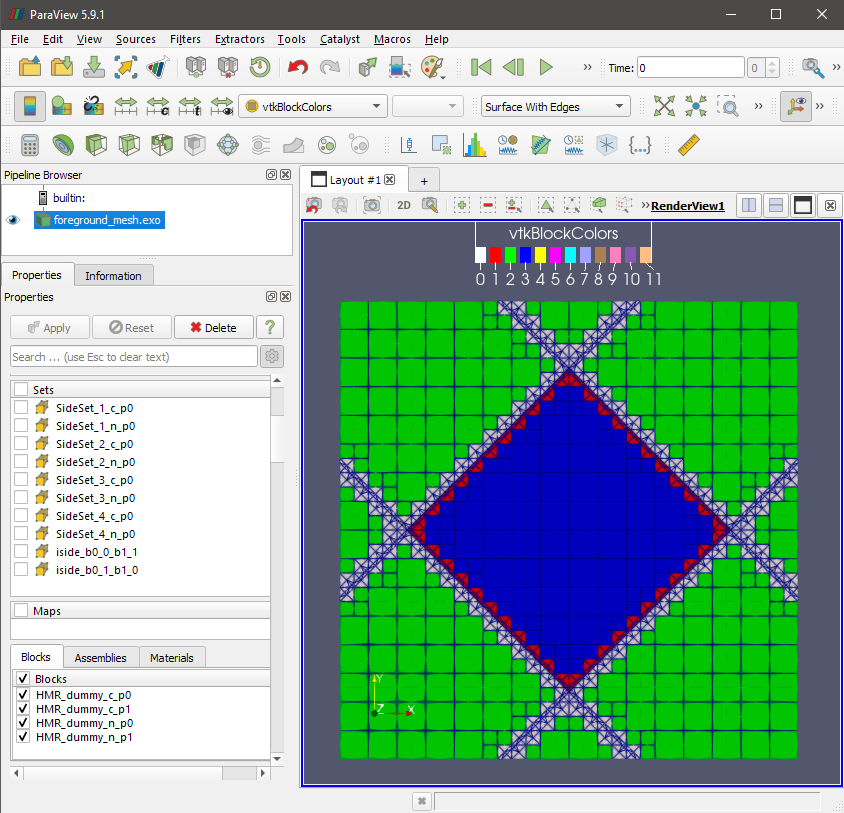
\includegraphics[width=12cm]{Figures/paraview_mesh_sets.png}
    \caption{Mesh blocks and sets written to the foreground mesh output for the \href{https://github.com/kkmaute/moris/blob/main/share/doc/mesh_generation/examples/Rotated_Square_Example.xml}{rotated square example} and how they are listed in ParaView.} 
    \label{fig:meshsets_paraview}
    \end{center}
\end{figure}

\begin{itemize}
    \item \textbf{Sets of facets of elements of a given Block that make up the boundary of the domain.} Each side of a domain is denoted using a \emph{side ordinal}. The convention for naming side ordinals, alongside other numbering conventions used in the EXODUS file format, can be found \href{https://sandialabs.github.io/seacas-docs/html/md_include_exodus_element_types.html}{here (\ExternalLink)}.
    The facets of the elements inside the block \texttt{HMR\_dummy\_c\_p0} that are part of the bottom, i.e. side ordinal $1$, of the domain are collected in the set \texttt{SideSet\_1\_c\_p0}. This allows boundary conditions to easily be imposed onto a given material along the various sides of the domain.
\end{itemize}

\refpar{future}{Future Developments} to the foreground mesh generation capabilities are to enable the triangulation of all elements even for locally refined foreground meshes. Further, enabling cubic foreground elements is possible.

% ------------------------------------------------------------------- %
\section{Extraction Operators}
\label{sec:tutorial_extraction_ops}

The \hyperref[eq:extraction_operator]{extraction operators} are computed per foreground element and \hyperlink{bspline_mesh_definition}{for each B-spline mesh defined}. For each B-spline mesh a separate HDF5 file is created that contains the B-spline mesh index with a prefix "\texttt{B}" in its name, 
\newline e.g. the files \texttt{Elemental\_Extraction\_Operators\_B0.hdf5} and
\newline \texttt{Elemental\_Extraction\_Operators\_B1.hdf5} contain the extraction operators with respect to B-spline mesh indices $0$ and $1$ respectively.

% \vspace{0.2cm}

\begin{figure}[h]
    \vspace{0.5cm}
    \begin{center}
    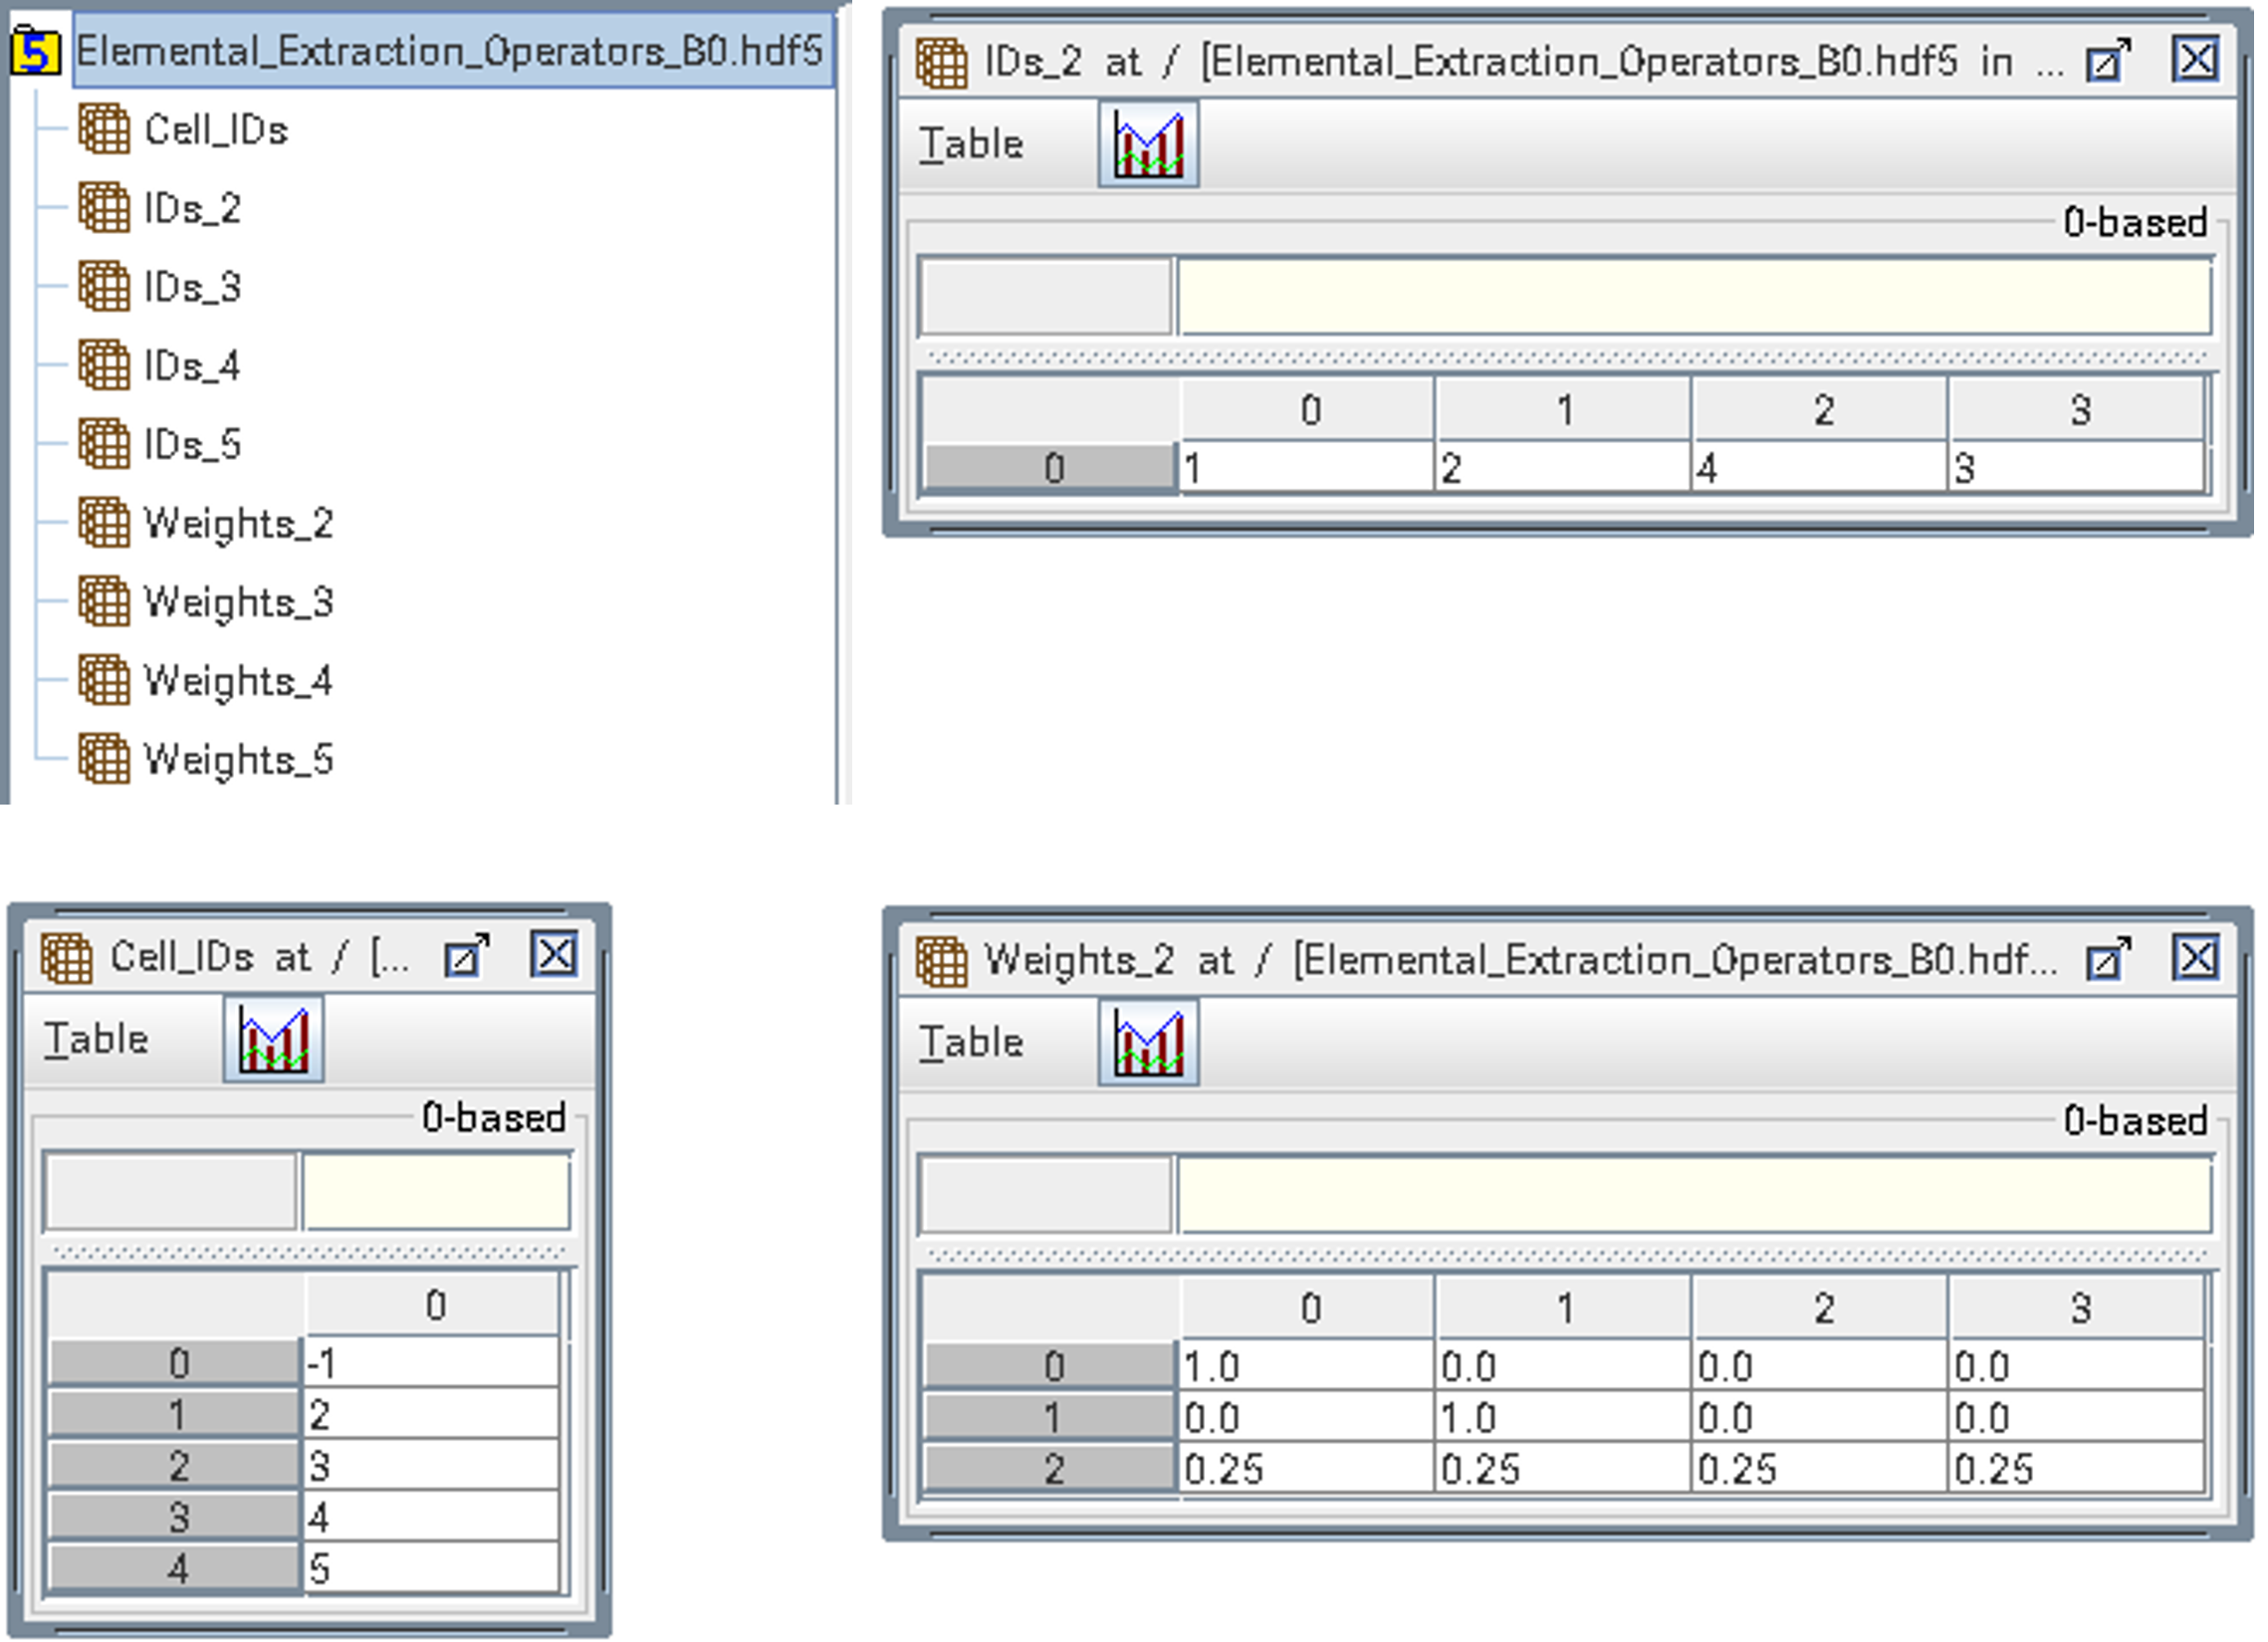
\includegraphics[width=12cm]{Figures/extraction_operator_output.png}
    \caption{Output of the extraction operators in HDF5 format for a foreground mesh consisting of four elements. The file contains a list of element IDs (bottom left), and for each element the extraction operator (bottom right) and an assembly map (top right).} 
    \label{fig:extraction_operator_output}
    \end{center}
\end{figure}

Each contains an array called \texttt{Cell\_IDs} that is an element index to ID array. An example is shown in \Cref{fig:extraction_operator_output}, bottom left. The index of an array entry represents the index of a foreground cell, the value of the entry is the ID. Note, the array may contain IDs whose value is $-1$ which indicates the corresponding element is not part of the foreground mesh outputted to the EXODUS file and can be ignored.

For each foreground element ID the extraction operator named \texttt{Weights\_<ID>} and a list of background basis function IDs named \texttt{IDs\_<ID>} are written to the HDF5 files. Examples are shown on the right in \Cref{fig:extraction_operator_output}. The weights are the extraction operators that are supposed to be applied to the elemental Jacobians, residuals, stiffness matrices, etc. as stated in equation \eqref{eq:transform_elemental} and demonstrated in \Cref{fig:assembly}. Once this operation is completed the ID vector is used to assemble the elemental matrix, or vector into the global system. In the elemental stiffness matrix example in \Cref{fig:assembly}, the entry in the second row and column, i.e. position $(2,3)$ would be assembled into position $(2,4)$ of the global stiffness matrix.

\begin{figure}[h]
    \begin{center}
    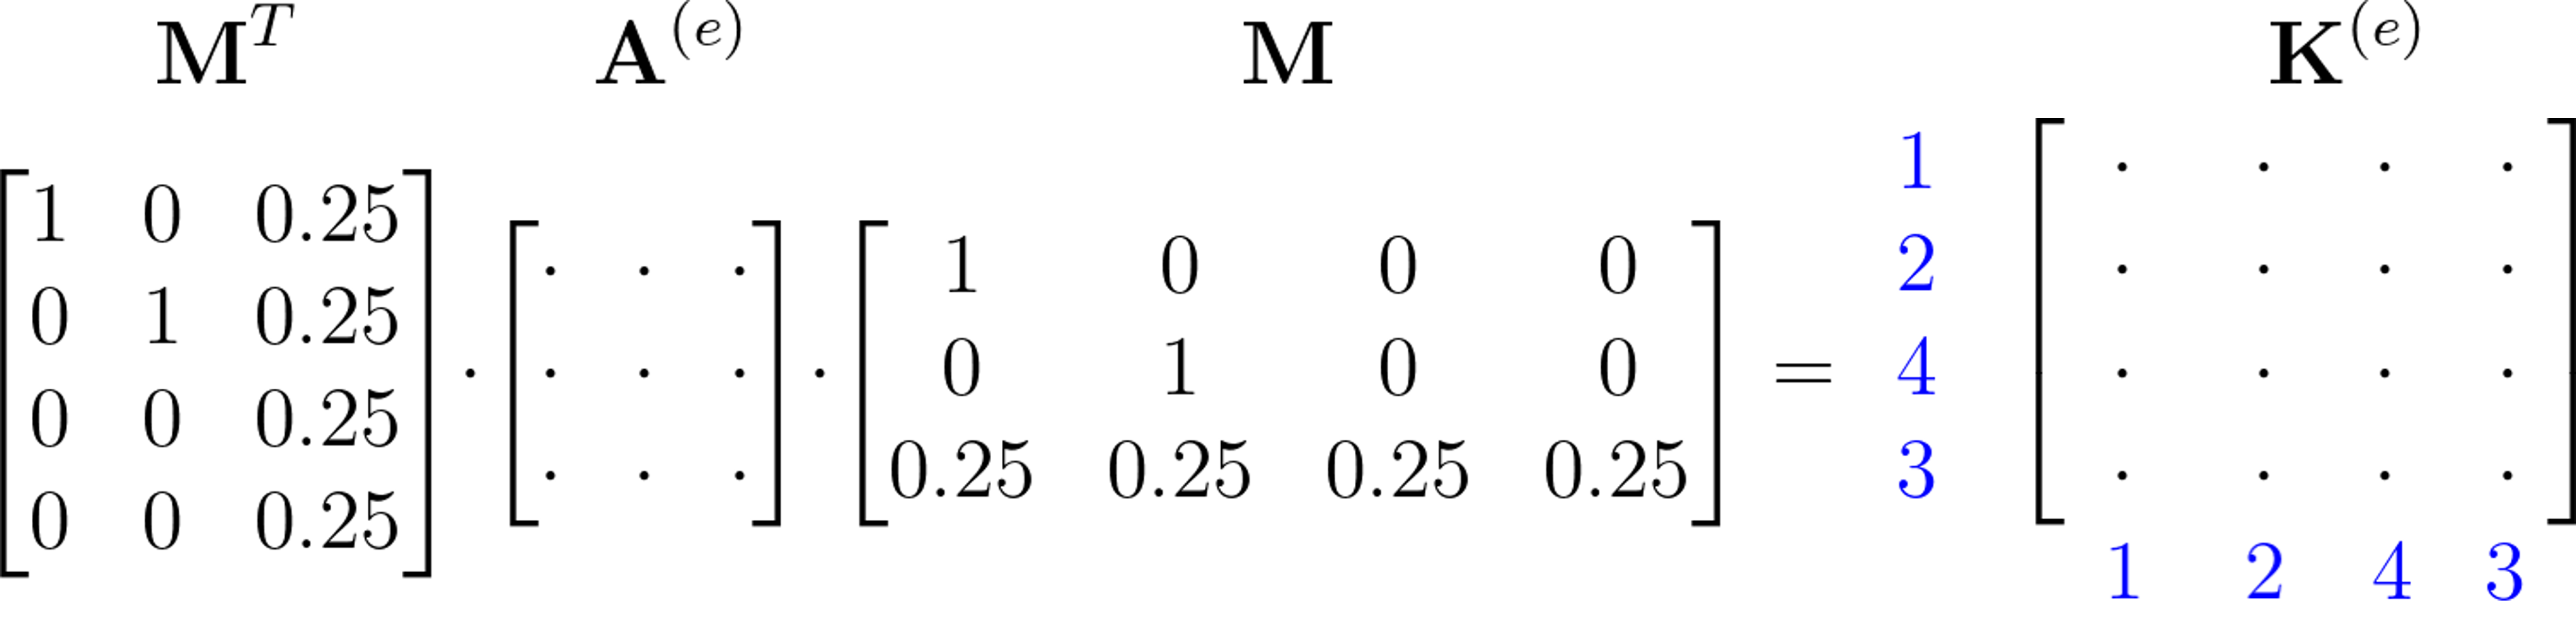
\includegraphics[width=12cm]{Figures/assembly.png}
    \caption{Projection of the elemental stiffness matrix $\bm{A}^{(e)}$ assembled on the Lagrange element into the background basis using the example extraction operators showm in in \Cref{fig:extraction_operator_output}. The blue arrays are the \texttt{IDs\_2} vector and serve as an assembly map.} 
    \label{fig:assembly}
    \end{center}
\end{figure}



